\documentclass{standalone}
\usepackage{tikz}
\usetikzlibrary{patterns, positioning}

\begin{document}
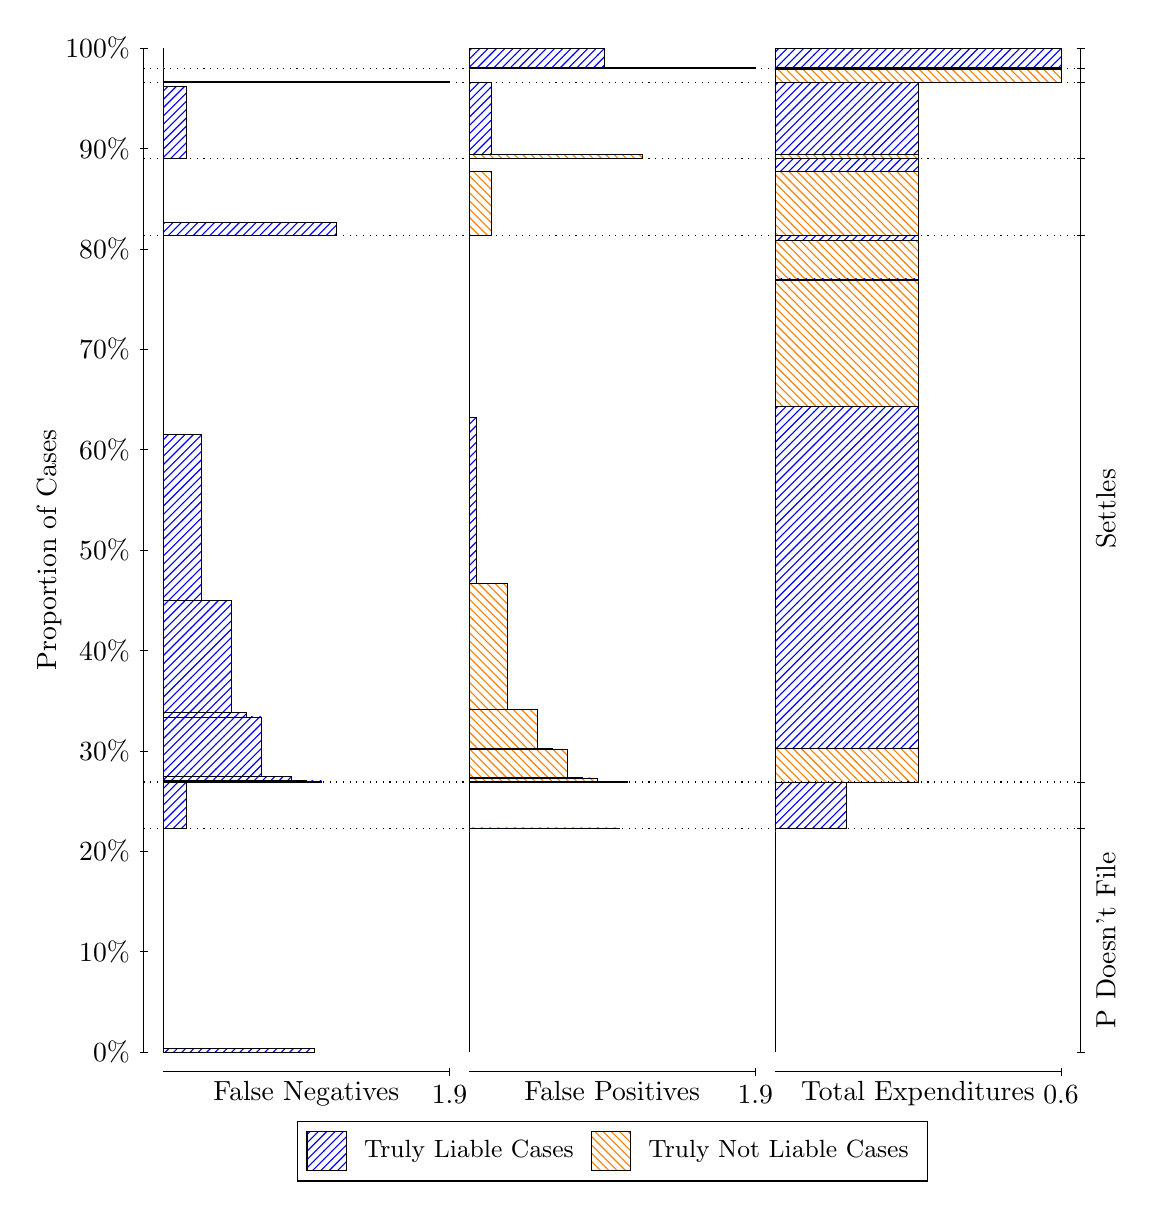
\begin{tikzpicture}
\draw[black, very thin] (1.5,1.75) -- (1.5,14.5);
\node[rotate=90, anchor=center] at (0.3, 8.125) {Proportion of Cases};
\draw[black, very thin] (1.45,1.75) -- (1.55,1.75);
\node[anchor=east] at (1.45, 1.75) {0\%};
\draw[black, very thin] (1.45,3.025) -- (1.55,3.025);
\node[anchor=east] at (1.45, 3.025) {10\%};
\draw[black, very thin] (1.45,4.3) -- (1.55,4.3);
\node[anchor=east] at (1.45, 4.3) {20\%};
\draw[black, very thin] (1.45,5.575) -- (1.55,5.575);
\node[anchor=east] at (1.45, 5.575) {30\%};
\draw[black, very thin] (1.45,6.85) -- (1.55,6.85);
\node[anchor=east] at (1.45, 6.85) {40\%};
\draw[black, very thin] (1.45,8.125) -- (1.55,8.125);
\node[anchor=east] at (1.45, 8.125) {50\%};
\draw[black, very thin] (1.45,9.4) -- (1.55,9.4);
\node[anchor=east] at (1.45, 9.4) {60\%};
\draw[black, very thin] (1.45,10.675) -- (1.55,10.675);
\node[anchor=east] at (1.45, 10.675) {70\%};
\draw[black, very thin] (1.45,11.95) -- (1.55,11.95);
\node[anchor=east] at (1.45, 11.95) {80\%};
\draw[black, very thin] (1.45,13.225) -- (1.55,13.225);
\node[anchor=east] at (1.45, 13.225) {90\%};
\draw[black, very thin] (1.45,14.5) -- (1.55,14.5);
\node[anchor=east] at (1.45, 14.5) {100\%};

\draw[black, very thin] (13.4,1.75) -- (13.4,14.5);
\draw[black, very thin] (13.35,1.75) -- (13.45,1.75);
\node[anchor=west] at (13.35, 1.75) {};
\draw[black, very thin] (13.35,4.5907) -- (13.45,4.5907);
\node[anchor=west] at (13.35, 4.5907) {};
\draw[black, very thin] (13.35,5.1782) -- (13.45,5.1782);
\node[anchor=west] at (13.35, 5.1782) {};
\draw[black, very thin] (13.35,12.117) -- (13.45,12.117);
\node[anchor=west] at (13.35, 12.117) {};
\draw[black, very thin] (13.35,13.099) -- (13.45,13.099);
\node[anchor=west] at (13.35, 13.099) {};
\draw[black, very thin] (13.35,14.063) -- (13.45,14.063);
\node[anchor=west] at (13.35, 14.063) {};
\draw[black, very thin] (13.35,14.243) -- (13.45,14.243);
\node[anchor=west] at (13.35, 14.243) {};
\draw[black, very thin] (13.35,14.5) -- (13.45,14.5);
\node[anchor=west] at (13.35, 14.5) {};

\draw[black, very thin, pattern color=blue, pattern=north east lines] (1.75,1.75) rectangle (3.6623,1.7918);
\draw[black, very thin, pattern color=orange, pattern=north west lines] (1.75,1.7918) rectangle (1.75,4.5907);
\draw[black, very thin, pattern color=blue, pattern=north east lines] (1.75,4.5907) rectangle (2.0368,5.1716);
\draw[black, very thin, pattern color=orange, pattern=north west lines] (1.75,5.1716) rectangle (1.75,5.1782);
\draw[black, very thin, pattern color=blue, pattern=north east lines] (1.75,5.1782) rectangle (3.7579,5.1927);
\draw[black, very thin, pattern color=blue, pattern=north east lines] (1.75,5.1927) rectangle (3.5667,5.195);
\draw[black, very thin, pattern color=blue, pattern=north east lines] (1.75,5.195) rectangle (3.3754,5.2469);
\draw[black, very thin, pattern color=blue, pattern=north east lines] (1.75,5.2469) rectangle (3.1842,5.2499);
\draw[black, very thin, pattern color=blue, pattern=north east lines] (1.75,5.2499) rectangle (2.993,6.0068);
\draw[black, very thin, pattern color=blue, pattern=north east lines] (1.75,6.0068) rectangle (2.8018,6.0664);
\draw[black, very thin, pattern color=blue, pattern=north east lines] (1.75,6.0664) rectangle (2.6105,7.4814);
\draw[black, very thin, pattern color=blue, pattern=north east lines] (1.75,7.4814) rectangle (2.4193,7.4822);
\draw[black, very thin, pattern color=blue, pattern=north east lines] (1.75,7.4822) rectangle (2.2281,9.5889);
\draw[black, very thin, pattern color=orange, pattern=north west lines] (1.75,9.5889) rectangle (1.75,12.117);
\draw[black, very thin, pattern color=blue, pattern=north east lines] (1.75,12.117) rectangle (3.9491,12.286);
\draw[black, very thin, pattern color=orange, pattern=north west lines] (1.75,12.286) rectangle (1.75,13.099);
\draw[black, very thin, pattern color=blue, pattern=north east lines] (1.75,13.099) rectangle (2.0368,14.01);
\draw[black, very thin, pattern color=orange, pattern=north west lines] (1.75,14.01) rectangle (1.75,14.063);
\draw[black, very thin, pattern color=blue, pattern=north east lines] (1.75,14.063) rectangle (5.3833,14.08);
\draw[black, very thin, pattern color=orange, pattern=north west lines] (1.75,14.08) rectangle (1.75,14.243);
\draw[black, very thin, pattern color=orange, pattern=north west lines] (1.75,14.243) rectangle (1.75,14.255);
\draw[black, very thin, pattern color=blue, pattern=north east lines] (1.75,14.255) rectangle (1.75,14.5);
\draw[black, very thin, pattern color=orange, pattern=north west lines] (5.6333,1.75) rectangle (5.6333,4.5489);
\draw[black, very thin, pattern color=blue, pattern=north east lines] (5.6333,4.5489) rectangle (5.6333,4.5907);
\draw[black, very thin, pattern color=orange, pattern=north west lines] (5.6333,4.5907) rectangle (7.5456,4.5973);
\draw[black, very thin, pattern color=blue, pattern=north east lines] (5.6333,4.5973) rectangle (5.6333,5.1782);
\draw[black, very thin, pattern color=orange, pattern=north west lines] (5.6333,5.1782) rectangle (7.6412,5.1854);
\draw[black, very thin, pattern color=orange, pattern=north west lines] (5.6333,5.1854) rectangle (7.45,5.1867);
\draw[black, very thin, pattern color=orange, pattern=north west lines] (5.6333,5.1867) rectangle (7.2588,5.2312);
\draw[black, very thin, pattern color=orange, pattern=north west lines] (5.6333,5.2312) rectangle (7.0675,5.2334);
\draw[black, very thin, pattern color=orange, pattern=north west lines] (5.6333,5.2334) rectangle (6.8763,5.5895);
\draw[black, very thin, pattern color=orange, pattern=north west lines] (5.6333,5.5895) rectangle (6.6851,5.6081);
\draw[black, very thin, pattern color=orange, pattern=north west lines] (5.6333,5.6081) rectangle (6.6851,5.6088);
\draw[black, very thin, pattern color=orange, pattern=north west lines] (5.6333,5.6088) rectangle (6.4939,6.1);
\draw[black, very thin, pattern color=orange, pattern=north west lines] (5.6333,6.1) rectangle (6.3026,6.1008);
\draw[black, very thin, pattern color=orange, pattern=north west lines] (5.6333,6.1008) rectangle (6.1114,7.7059);
\draw[black, very thin, pattern color=blue, pattern=north east lines] (5.6333,7.7059) rectangle (5.7289,9.8126);
\draw[black, very thin, pattern color=blue, pattern=north east lines] (5.6333,9.8126) rectangle (5.6333,12.117);
\draw[black, very thin, pattern color=orange, pattern=north west lines] (5.6333,12.117) rectangle (5.9202,12.93);
\draw[black, very thin, pattern color=blue, pattern=north east lines] (5.6333,12.93) rectangle (5.6333,13.099);
\draw[black, very thin, pattern color=orange, pattern=north west lines] (5.6333,13.099) rectangle (7.8325,13.153);
\draw[black, very thin, pattern color=blue, pattern=north east lines] (5.6333,13.153) rectangle (5.9202,14.063);
\draw[black, very thin, pattern color=orange, pattern=north west lines] (5.6333,14.063) rectangle (5.6333,14.226);
\draw[black, very thin, pattern color=blue, pattern=north east lines] (5.6333,14.226) rectangle (5.6333,14.243);
\draw[black, very thin, pattern color=orange, pattern=north west lines] (5.6333,14.243) rectangle (9.2667,14.255);
\draw[black, very thin, pattern color=blue, pattern=north east lines] (5.6333,14.255) rectangle (7.3544,14.5);
\draw[black, very thin, pattern color=orange, pattern=north west lines] (9.5167,1.75) rectangle (9.5167,4.5489);
\draw[black, very thin, pattern color=blue, pattern=north east lines] (9.5167,4.5489) rectangle (9.5167,4.5907);
\draw[black, very thin, pattern color=orange, pattern=north west lines] (9.5167,4.5907) rectangle (10.425,4.5973);
\draw[black, very thin, pattern color=blue, pattern=north east lines] (9.5167,4.5973) rectangle (10.425,5.1782);
\draw[black, very thin, pattern color=orange, pattern=north west lines] (9.5167,5.1782) rectangle (11.333,5.6081);
\draw[black, very thin, pattern color=blue, pattern=north east lines] (9.5167,5.6081) rectangle (11.333,9.9478);
\draw[black, very thin, pattern color=orange, pattern=north west lines] (9.5167,9.9478) rectangle (11.333,11.553);
\draw[black, very thin, pattern color=blue, pattern=north east lines] (9.5167,11.553) rectangle (11.333,11.567);
\draw[black, very thin, pattern color=orange, pattern=north west lines] (9.5167,11.567) rectangle (11.333,12.06);
\draw[black, very thin, pattern color=blue, pattern=north east lines] (9.5167,12.06) rectangle (11.333,12.117);
\draw[black, very thin, pattern color=orange, pattern=north west lines] (9.5167,12.117) rectangle (11.333,12.93);
\draw[black, very thin, pattern color=blue, pattern=north east lines] (9.5167,12.93) rectangle (11.333,13.099);
\draw[black, very thin, pattern color=orange, pattern=north west lines] (9.5167,13.099) rectangle (11.333,13.153);
\draw[black, very thin, pattern color=blue, pattern=north east lines] (9.5167,13.153) rectangle (11.333,14.063);
\draw[black, very thin, pattern color=orange, pattern=north west lines] (9.5167,14.063) rectangle (13.15,14.226);
\draw[black, very thin, pattern color=blue, pattern=north east lines] (9.5167,14.226) rectangle (13.15,14.243);
\draw[black, very thin, pattern color=orange, pattern=north west lines] (9.5167,14.243) rectangle (13.15,14.255);
\draw[black, very thin, pattern color=blue, pattern=north east lines] (9.5167,14.255) rectangle (13.15,14.5);
\draw[black, dotted] (1.5,4.5907) -- (13.4,4.5907);
\draw[black, dotted] (1.5,5.1782) -- (13.4,5.1782);
\draw[black, dotted] (1.5,12.117) -- (13.4,12.117);
\draw[black, dotted] (1.5,13.099) -- (13.4,13.099);
\draw[black, dotted] (1.5,14.063) -- (13.4,14.063);
\draw[black, dotted] (1.5,14.243) -- (13.4,14.243);
\draw[black, very thin] (1.75,1.5) -- (5.3833,1.5);
\node[anchor=north] at (3.5667, 1.5) {False Negatives};
\draw[black, very thin] (5.3833,1.45) -- (5.3833,1.55);
\node[anchor=north] at (5.3833, 1.45) {1.9};

\draw[black, very thin] (5.6333,1.5) -- (9.2667,1.5);
\node[anchor=north] at (7.45, 1.5) {False Positives};
\draw[black, very thin] (9.2667,1.45) -- (9.2667,1.55);
\node[anchor=north] at (9.2667, 1.45) {1.9};

\draw[black, very thin] (9.5167,1.5) -- (13.15,1.5);
\node[anchor=north] at (11.333, 1.5) {Total Expenditures};
\draw[black, very thin] (13.15,1.45) -- (13.15,1.55);
\node[anchor=north] at (13.15, 1.45) {0.6};

\node[black, centered, rotate=90] at (13.72, 3.1704) {P Doesn't File};

\node[black, centered, rotate=90] at (13.72, 8.6474) {Settles};





\draw (7.449999999999999,1.5) node[draw=none] (baseCoordinate) {};
\begin{scope}[align=center]
        \matrix[scale=0.5, draw=black, below=0.5cm of baseCoordinate, nodes={draw}, column sep=0.1cm]{
            \node[rectangle, draw, minimum width=0.5cm, minimum height=0.5cm, pattern=north east lines, pattern color=blue] {}; &
            \node[draw=none, font=\small] (B) {Truly Liable Cases}; &
            \node[rectangle, draw, minimum width=0.5cm, minimum height=0.5cm, pattern=north west lines, pattern color=orange] {}; &
            \node[draw=none, font=\small] (B) {Truly Not Liable Cases}; \\
            };
\end{scope}

\end{tikzpicture}
\end{document}